\chapter{Introducción} 
\label{chap:intro}

\vspace{-0.2cm}

\lsection{Motivación del proyecto}

Los sistemas domóticos por lo general utilizan una arquitectura centralizada: un controlador (bridge) es el encargado de enviar y recibir información de los dispositivos domóticos y las interfaces.
 Se utilizan sistemas centralizados debido a que abaratan mucho el coste de los dispositivos domóticos, así los dispositivos tienen poca electrónica y programación, y la responsabilidad principal
 reside en el bridge. Este enfoque tiene sentido cuando se trata de muchos dispositivos en un hogar, que es el caso ideal, si solo tuviésemos un sensor carecería de sentido tener un sensor y un bridge para manejarlo.

El problema principal que existe con los sistemas centralizados se encuentra en la \textbf{compatibilidad} entre dispositivos y bridges.
Por lo que he observado~\cite{article:EstadoDelArte}, todavía falta mucha estandarización en el
ámbito de la domótica: cada fabricante usa sus medios y protocolos haciendo incompatibles bridges y dispositivos. Además, estos dispositivos no suelen ser 
muy asequibles. Por lo tanto, nos encontramos ante la necesidad de comprar todos los dispositivos de una misma marca o tener muchos bridges, lo que nos obligaría a manejar cada
dispositivo desde su correspondiente bridge.

La domótica puede hacernos la vida en el hogar mucho más sencilla, ayudándonos a ahorrar tiempo y dinero que podremos invertir en otras cosas. Los hogares todavía están muy poco automatizados, y mi principal motivación ha sido acercar la domótica 
a las personas y aprender acerca de ella. Gracias a nuestro sistema manejamos todos los dispositvos a través de un solo bridge de manera sencilla y eficaz.

\newpage
\lsection{Objetivos y enfoque}

El objetivo último de nuestro proyecto es desarrollar un sistema que sea capaz de recibir y enviar información de dispositivos domóticos y sea capaz de interactuar con el cliente. 

Los \textbf{requisitos} que debe cumplir nuestro sistema son:
\begin{itemize}
  \item \underline{Ligero.} Un bridge no debería necesitar demasiada capacidad de procesamiento y de memoria, y es necesario que no sea muy costoso, por lo tanto, la ligereza es requisito indispensable.
  \item \underline{Compatibilidad.} Necesitamos que nuestro bridge no sea únicamente compatible con un tipo de sensor, o un modelo de cámara
  \item \underline{Interfaz sencilla y adaptable a cualquier dispositivo.} Necesitamos que la interfaz de nuestro bridge sea compatible con cualquier dispositivo sin perder funcinalidad.
  \item \underline{Seguridad.} La seguridad en la domótica es algo indispensable, confío en que el día de mañana incluso las cerraduras de nuestras casas serán automáticas, y no podemos dejar la responsabilidad de la seguridad
  de nuestra a casa a un sistema con vulnerabilidades de seguridad.
  \item \underline{Escalable.} Nuestro sistema ha de ser escalable y debemos pensar en todo momento en ampliaciones y trabajos futuros. La domótica evoluciona a pasos agigantados y podríamos añadir funcionalidades a nuestro 
  sistema practicamente a diario. No obstante, es necesario acotar firmemente los límites de nuestro proyecto para ceñirnos a las horas que corresponden a un TFG, aunque debemos tener muy en cuenta en todo momento trabajos futuros y ampliaciones.
  Además, debemos tener en cuenta la escalabilidad: domótica en un hospital, en una ciudad...etc.
\end{itemize}


\lsection{Metodología y plan de trabajo}

Debido a que los capítulos del documento coinciden con las fases de ciclo de vida de nuestro proyecto, es importante explicar la metodología antes de explicar la estructura del documento.
\par
La metodología que se ha utilizado para el desarrollo de nuestro proyecto es una metodología tradicional con un ciclo de vida en cascada. Se utilizarán las siguientes etapas, que se realizarán una detrás de otra (en cascada):

\begin{itemize}
\item\underline{Requisitos}: en esta fase se analizarán los requisitos y las necesidades del sistema a desarrollar. Un buen análisis guía un buen desarrollo, mientras que un análisis mal hecho
puede significar que el proyecto tenga retrasos, fallos e incluso su cancelación.
\item\underline{Diseño}: se detallarán la arquitectura, los componentes y los subsistemas que formarán parte de nuestro sistema final, así como la interacción entre ellos.
\item\underline{Implementación}: esta es la primera fase en la que se comienza a materializar nuestro sistema. Se definirán las tecnologías a utilizar y se llevará a cabo el desarrollo de un sistema que siga
el diseño realizado y cumpla los requisitos descritos.
\item\underline{Verificación}: también conocida como fase de pruebas, en esta fase se probará que nuestro sistema cumpla con los requisitos especificados. Se utiliza para detectar posibles errores.
\item\underline{Mantenimiento}: durante esta fase se implanta el sistema y se atienden posibles incidencias que puedan surgir a lo largo del uso del mismo.

\end{itemize}

\begin{figure}[H]
\centering
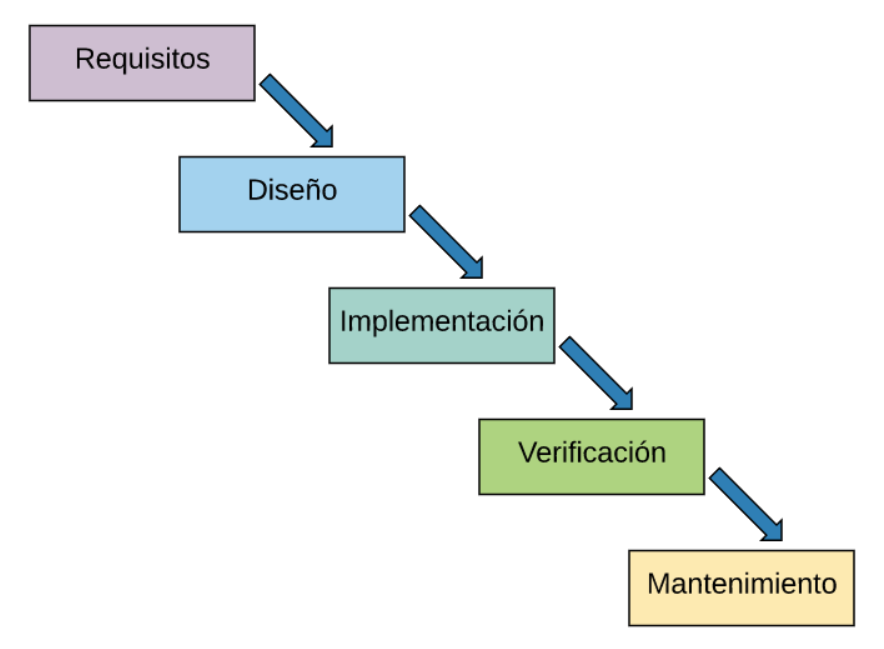
\includegraphics[width=4.00in]{images/desarrollo_cascada.PNG}
\caption{Las etapas del modelo en cascada.
 Recuperado de: https://openclassrooms.com/en/courses/4309151-gestiona-tu-proyecto-de-desarrollo/4538221-en-que-consiste-el-modelo-en-cascada}
\label{fig:tecnologias_populares}
\end{figure}


\lsection{Estructura del documento}

A lo largo del siguiente documento se irán explicando todas las fases del ciclo de vida de nuestro proyecto, además de tener una fase previa de análisis de estado del 
arte y una fase posterior de trabajos futuros y conclusiones:
\begin{itemize}
\item\textbf{Estado del arte - \autoref{chap:estadodelarte}}: breve introducción y análisis de la domótica en la actualidad.
\item\textbf{Análisis y diseño - \autoref{chap:analisisydisenosistema}}: a lo largo del capítulo tres se analizan los requisitos de nuestra aplicación y se diseña la arquitectura del sistema.
\item\textbf{Desarrollo del sistema - \autoref{chap:desarrollosistema}}: en este capítulo se describirán las tecnologías utilizadas para el desarrollo del sistema, y se detallarán 
algunos aspectos técnicos acerca de la implementación.
\item\textbf{Pruebas - \autoref{chap:pruebas}}: en este capítulo se detallarán las pruebas realizadas para comprobar el correcto funcionamiento
de nuestro sistema y la detección de posibles bugs.
\item\textbf{Trabajos futuros - \autoref{chap:trabajofuturo}}: análisis de posibles trabajos futuros para nuestro HUB.
\item\textbf{Conclusiones - \autoref{chap:conclusiones}}: conclusiones obtenidas a lo largo del trabajo.
\end{itemize}


\newpage \thispagestyle{empty} % Página vacía 